\subsection{Controller implementation (Mikkel) }
As mentioned in the Design section \ref{sec:securitydesign}, we divided the control into three classes, \texttt{BankApplication}, \texttt{DefaultServlet} and \texttt{DatabaseProtocol}. 

\begin{itemize}
    \item \texttt{BankApplication} handles the internal logic, comprised of Java code. Having a controller dedicated to the internal logic made it very easy to extend basic functionality throughout the coding process, and troubleshoot logical errors.
    \item \texttt{DefaultServlet} handles the webpages, and is thus a fairly simple controller. Its main responsibility is receiving HTTP requests, taking actions accordingly, and sending HTTP responses to the View pages.
    \item \texttt{DatabaseProtocol} handles the requests to the database and SQL statements.
\end{itemize}
  
The hierarchy between controllers goes as follows: \texttt{DefaultServlet} $\rightarrow$ \texttt{BankApplication} $\rightarrow$ \texttt{DatabaseProtocol}. This structure was chosen, as it corresponds with the way actions are carried out, starting through the interface $\rightarrow$ processed by internal logic $\rightarrow$ committing changes to the database. The control classes thus correspond to the different levels of abstraction, with the extremes being \texttt{DefautlServlet} knows what the user wants to do (but not how to do it) and \texttt{DatabaseProtocol} knows the data, but not what the user wants to do. This creates a structure where \texttt{DefaultServlet} is close to the View-part of the program, and \texttt{DatabaseProtocol} is close to the Model-part, more specifically the database. \texttt{BankApplication} acts as the bridge between the two, while also handling the Model-part of the program not in the database.

\begin{figure}[H]
\centering
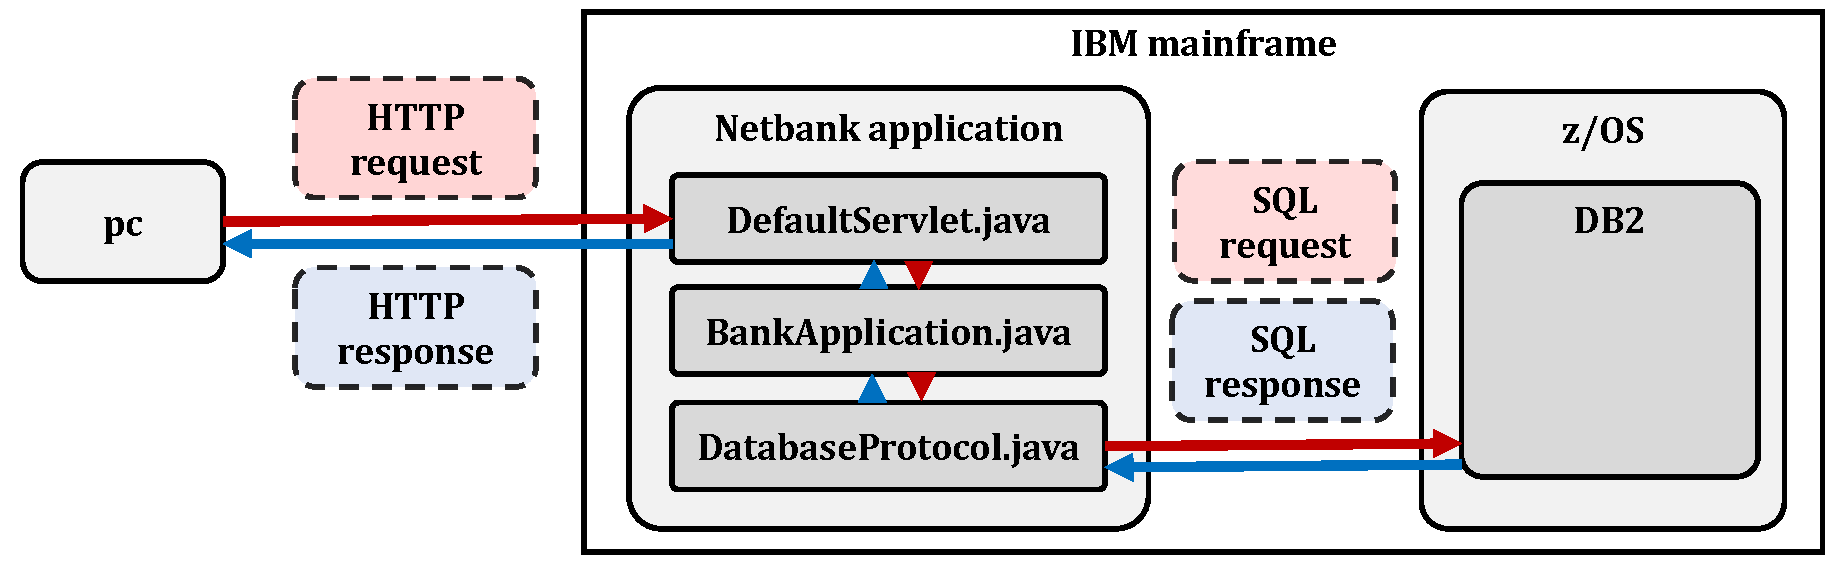
\includegraphics[width = 0.9\textwidth]{figures/interaction_transfer.pdf}
\caption{Control flow in the program, and how the three controllers interact with the program.}
\label{fig:interactiontransfer}
\end{figure}